% !TeX TS-program = txs:///duck
\documentclass{standalone}

\usepackage{tikzducks}

\begin{document}
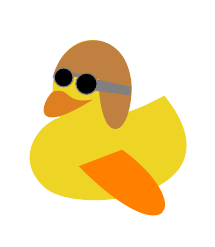
\begin{tikzpicture}
\duck

% wing
\path (0.1,-0.15) rectangle (2.1,2.12);
\begin{pgfinterruptboundingbox}
	\fill[orange] (0.7331,0.5229) .. controls (1.8688,-0.6326) and (2.2337,0.0383) .. (1.2819,0.7331) -- cycle;
\end{pgfinterruptboundingbox}

\fill[brown] (1.3848,1.6771) .. controls (1.2665,2.2823) and (0.5559,2.2697) .. (0.4000,1.6455) .. controls (0.5711,1.6714) and (0.8503,1.6562) .. (0.9926,1.6247) .. controls (0.9703,1.4641) and (1.0307,1.0718) .. (1.1444,1.0104) .. controls (1.3485,0.9002) and (1.4461,1.4498) .. (1.3848,1.6771) -- cycle;

\fill[gray] (0.9153,1.4857) -- (0.9472,1.6278) -- (1.3926,1.5288) -- (1.3840,1.4228) -- cycle;
\fill[gray] (0.6484,1.6773) -- (0.6601,1.7155) -- (0.7558,1.6863) -- (0.7441,1.6480) -- cycle;

\draw[gray,fill=black] (0.83,1.57) circle (0.135);
\draw[gray,fill=black] (0.54,1.65) circle (0.12);


\end{tikzpicture}
\end{document}